\documentclass[10pt,a4paper]{beamer}
\usepackage[utf8]{inputenc}
\usepackage{amsmath}
\usepackage{amsfonts}
\usepackage{amssymb}
\usepackage[labelformat=empty]{subcaption}
\usepackage{graphicx}
\usepackage[dutch]{babel}
\usepackage{lmodern}
\usepackage{epstopdf}
\usepackage{ulem}
\usepackage{graphicx}
\usepackage[labelformat=empty]{caption}

\author{Falco Peijnenburg}
\usetheme{Warsaw}
%\setbeamertemplate{footline}{\insertframenumber/\inserttotalframenumber}


\title[Git crash course\hspace{40mm} \insertframenumber/\inserttotalframenumber]{Git crash course}


\begin{document}

% Title frame
\frame{\titlepage}

\setcounter{tocdepth}{1}
% Table of contents
\begin{frame}
\frametitle{Table of contents}
\tableofcontents[]
\end{frame}


\section{About git}
\subsection{What is git}
\begin{frame}{What is git}
\begin{itemize}
\item VCS (Version control systems)
\item SCM (Source code management)
\item Originally made by Linus Torvalds
\item Basically it makes your life easier when programming
\end{itemize}
\end{frame}

\subsection{Advantages git}

\begin{frame}{By itself}
\begin{itemize}
\item Distributed
\item Fast (both in speed of commands and workflow)
\item You can work offline
\item Forces you to have proper, structured workflow (and \textit{yes} this is good for everyone)
\item Has many features that are actually useful
\item It's useful even for people who work alone
\item Amazing branching implementation

\end{itemize}
\end{frame}
% multiple remotes, no problem

\begin{frame}{Compared to Dropbox/Google Drive}
\begin{itemize}
\item No more copying folders for an experimental feature/recode (seriously, this is ridiculous)
\item Work simultaneously without the \textit{utter} chaos of conflict files
\item You can very easily revert if you make a mistake
\item Better tracking of changes
\item The ability to find out when and by whom a bug was introduced
\end{itemize}
\end{frame}

\begin{frame}{Compared to SVN}
\begin{itemize}
\item Faster, by far
\item Branching isn't terrible
\item Cli isn't terrible
\item SVN is \textit{very} limited in features once you know what git can do
\item You can have multiple remotes (will be explained later)
\item Pull requests
\item Git has no single point of failure.
\item Integrity checking (minor)
\item ``\textit{Take CVS as an example of what not to do; if in doubt, make the exact opposite decision.}'' (Torvalds)
\item (SVN's original slogan was CVS done right)

\end{itemize}
\end{frame}


\section{Getting started with git}


\subsection{How to install}
\begin{frame}{How to install}
\begin{itemize}
\item Linux:
\begin{itemize}
\item apt-get install git
\item pacman -S git
\item yum install git
\item ...
\end{itemize}
\item Windows/Mac: \href{http://git-scm.com/downloads}{\color{blue}http://git-scm.com/downloads}

When installing, use advanced context menu integration. Use default settings in other screens
\end{itemize}
\end{frame}

\subsection{Opening git bash}
\begin{frame}{Opening git bash}
Linux/Mac
\begin{itemize}
\item Open the terminal
\item cd to the right folder
\end{itemize}

Windows:
\begin{itemize}
\item Right click a folder
\item Click ``Git Bash''. Don't use the normal command prompt.
\end{itemize}

Tip: Leave the terminal open in the background while you work.


\end{frame}

\subsection{Setting up}
\begin{frame}[fragile]{Setting up}
\begin{itemize}
\item Git needs to know your name and email address.
\item It uses that information to assign an author to a commit.
\end{itemize}

\begin{verbatim}
git config --global user.name "John Doe"
git config --global user.email "johndoe@example.com"
\end{verbatim}

\begin{itemize}
\item You will need a public/private keypair to communicate with a git server through ssh. Follow this guide:
\item \href{http://git-scm.com/downloads/guis}{\color{blue}https://help.github.com/articles/generating-ssh-keys}
\end{itemize}
\end{frame}

\subsection{Making a repository}
\begin{frame}[fragile]{Making a repository}
Two options:

\begin{itemize}
\item Start your own empty local repository.
\end{itemize}

	\begin{verbatim}
	git init
	\end{verbatim}

\begin{itemize}
\item Clone the repository from a server.
\end{itemize}

	\begin{verbatim}
	git clone URL_HERE
	git clone git@github.com:FPtje/DarkRP.git
	\end{verbatim}
\end{frame}


\section{Basic git structure}
\subsection{Basic git structure}
\begin{frame}{Basic git structure}
A git repository has three states
\begin{itemize}
\item Working directory
\item Staging area
\item Git directory
\end{itemize}
\end{frame}

\begin{frame}[plain]
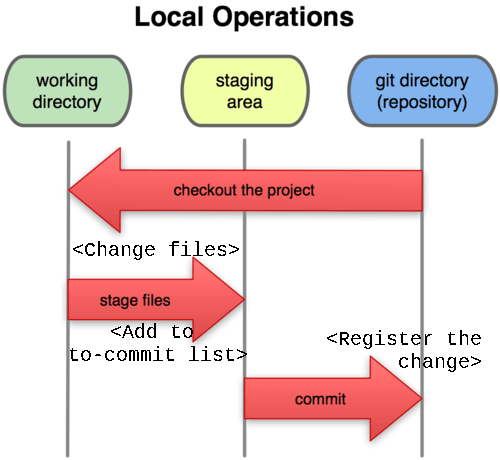
\includegraphics[width=\linewidth]{threeStates.png}
\end{frame}

\begin{frame}[plain]
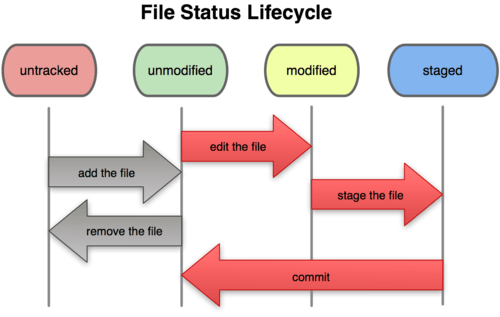
\includegraphics[width=\linewidth]{fileLifeCycle.png}
\end{frame}

\subsection{Initial commit}
\begin{frame}{Initial commit}
Applies only to an empty repository (created by git init)
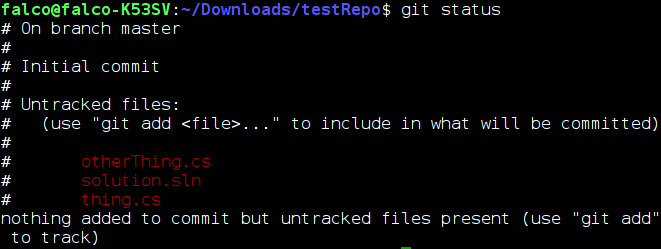
\includegraphics[width=\linewidth]{gitStatus1.png}
\end{frame}

\subsection{Adding/removing files}
\begin{frame}
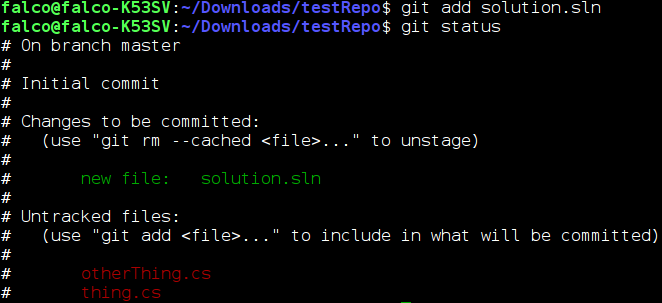
\includegraphics[width=\linewidth]{gitAdd.png}
\end{frame}

\begin{frame}
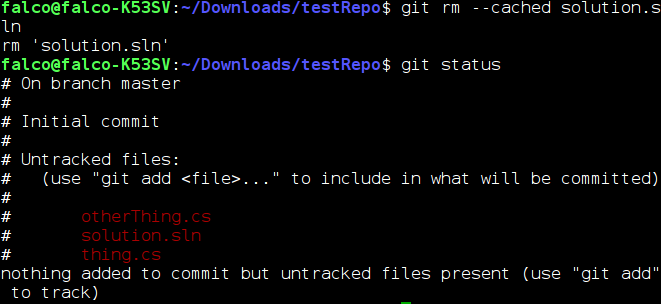
\includegraphics[width=\linewidth]{gitrmcached.png}
\end{frame}

\begin{frame}
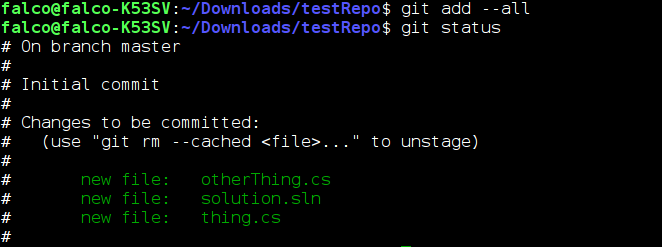
\includegraphics[width=\linewidth]{gitaddall.png}
\end{frame}

\begin{frame}
There's also:
\begin{itemize}
\item git mv file location -- Move or rename a file. Same syntax as mv command.
\item .gitignore -- a file that contains regex patterns of files that git should leave alone. Use this for executables, .obj files etc.
\end{itemize}
Tip for .gitignore files:
\href{http://git-scm.com/downloads/guis}{\color{blue}https://github.com/github/gitignore}
\end{frame}

\subsection{Committing changes}
\begin{frame}[fragile]{Committing changes}
\begin{itemize}
\item Commit everything that's staged using git commit
\item Every commit message \textit{must} have a commit message! Tell git what you've done!
\end{itemize}
\begin{verbatim}
-- Opens vi or nano by default for the commit message:
git commit
-- Inline commit message:
git commit -m "Message here"
-- Skip staging of modified files
git commit -a -m "Message here"
git commit -am "Message here"
\end{verbatim}
\begin{itemize}
\item You cannot skip the staging of new files. Add them manually.
\end{itemize}
\end{frame}

\begin{frame}
Running the command:
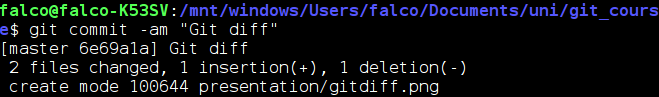
\includegraphics[width=\linewidth]{gitcommitdone.png}

Some of the info stored in the commit:
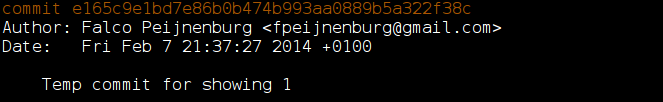
\includegraphics[width=\linewidth]{gitlogcommit.png}
\end{frame}

\section{Further commits}

\subsection{git diff}
\begin{frame}
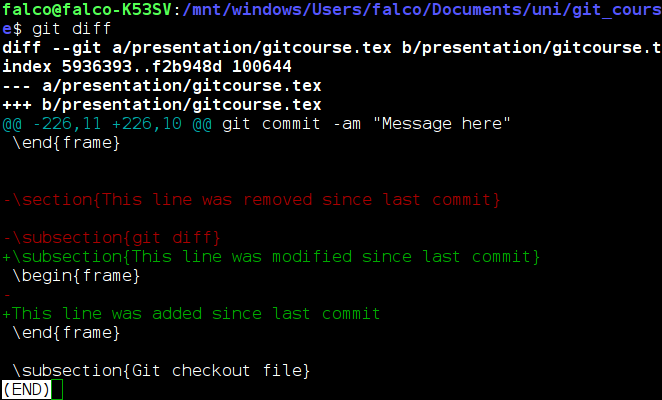
\includegraphics[width=\linewidth]{gitdiff.png}
\end{frame}

\subsection{git checkout file}
\begin{frame}{git checkout file}
\begin{itemize}
\item Undoes all the changes made to a file since last commit.
\item Doesn't leave a message
\end{itemize}

\includegraphics[width=\linewidth]{gitcheckoutfile.png}
\end{frame}

\subsection{git reset}
\begin{frame}[fragile]{git reset}
\begin{itemize}
\item useful when you've messed up the files in your working directory
\item Reset every file in your working directory to the last revision:

\begin{verbatim}
git reset --hard HEAD
\end{verbatim}
\item git reset can do many other things, but you shouldn't want to use most of those things.
\item HEAD will be explained later
\end{itemize}
\end{frame}

\subsection{git log}
\begin{frame}{git log}
\centerline{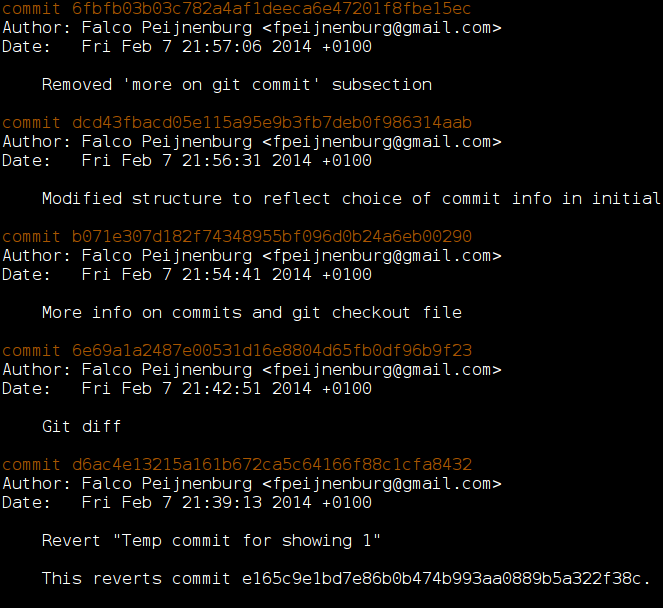
\includegraphics[height=6cm]{gitlog.png}}
\end{frame}

\subsection{gitk}
\begin{frame}
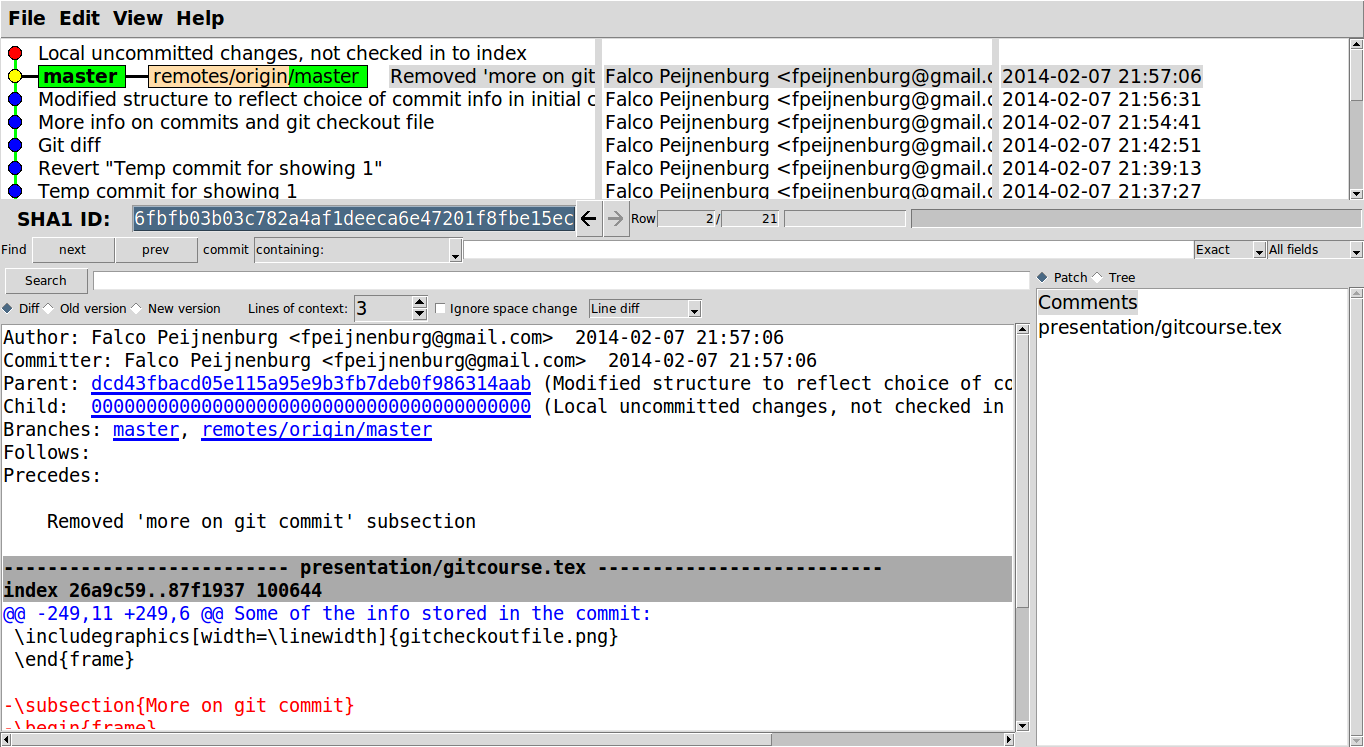
\includegraphics[width=\linewidth]{gitk.png}
\end{frame}

\subsection{git show}
\begin{frame}[fragile]{git show}
\begin{verbatim}
git show
\end{verbatim}
\begin{itemize}
\item Shows last commit information + diff
\end{itemize}

\begin{verbatim}
git show Hash_here
git show 7251b9
\end{verbatim}
\begin{itemize}
\item Shows commit info and diff of given commit
\item You can show any git object (commits, branches, stashes)
\item You don't have to use the full hash
\end{itemize}
\end{frame}


\section{The tree of commits}

\subsection{Master branch}
\begin{frame}{Master Branch}
\begin{itemize}
\item This is what we've been committing to so far.
\item Much like a linked list
\item Every commit knows its parent(s)
\item Tip of the branch is called HEAD, then HEAD\^{}, HEAD\~{}2, ...
\end{itemize}
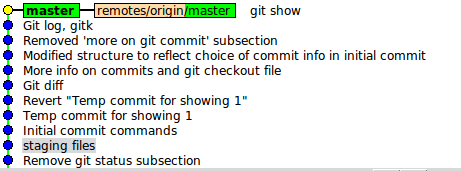
\includegraphics[width=\linewidth]{masterbranch.png}
\end{frame}

\subsection{Creating your own branch}
\begin{frame}[fragile]{Creating your own branch}
\begin{verbatim}
git branch branchname
git checkout branchname
\end{verbatim}
\begin{itemize}
\item Mind the git checkout command. It might be confusing at first.
\item Shorter:
\end{itemize}

\begin{verbatim}
git checkout -b branchname
\end{verbatim}
\begin{itemize}
\item Official definition of checkout:
\item \textit{Checkout a branch or paths to the working tree}
\end{itemize}
\end{frame}

\subsection{Switching branches}
\begin{frame}[fragile]{Switching branches}
\begin{verbatim}
git checkout master
git checkout branchname
git checkout otherBranch
\end{verbatim}
\begin{itemize}
\item You can switch from any branch to any other branch
\item Might fail if you have uncommitted changes
\end{itemize}
\end{frame}

\subsection{Merging branches}
\begin{frame}[fragile]{Merging branches}
\begin{verbatim}
git checkout mergeTo
git merge mergeFrom
\end{verbatim}
\begin{itemize}
\item Make sure you're on the right branch first
\item Conflicts may occur when merging
\item A new special merge commit will be created with \textit{two} parent commits
\item All commits from the mergeFrom branch will be visible in the mergeTo branch
\end{itemize}
\end{frame}

\subsection{Removing branches}
\begin{frame}[fragile]{Removing branches}
\begin{verbatim}
git branch -d branchname
git branch -D branchname
\end{verbatim}
\begin{itemize}
\item The former will fail if there are unmerged changes
\item The latter will not, so be careful
\end{itemize}
\end{frame}


\section{Resolving conflicts}

\subsection{What is a conflict}
\begin{frame}{What is a conflict}
\begin{itemize}
	\item Harry and Larry are working on a website
	\item Harry and Larry both edit the footer div of the main web page
	\item Harry is working on master
	\item Larry is working on the refactor branch he created
	\item After a while Larry is done working and wants to merge refactor into master
\end{itemize}
\end{frame}

\begin{frame}[fragile]
\begin{verbatim}
$ git merge refactor
Auto-merging index.html
CONFLICT (content): Merge conflict in index.html
Automatic merge failed; fix conflicts and then commit
the result.
\end{verbatim}
\begin{itemize}
	\item Two people edited the same file in the same place
	\item What should git do?
	\begin{itemize}
	\item Use Harry's version?
	\item Use Larry's version?
	\item Use a combination of both versions?
	\item Use neither version?
	\end{itemize}

	\item Another kind of conflict: Larry modifies a file that Harry removed. Use modified or removed?
\end{itemize}
\end{frame}

\subsection{Fixing the conflicts in the file}
% It's not a mess
\begin{frame}[fragile]{Fixing the conflicts in the file}
\begin{itemize}
\item Git will edit the files that have the conflicts
\item ``conflict markers'' will be added.
\item git status and git diff will tell you which files are conflicted.
\item Fix the conflicts in visual studio or your favourite text editor.
\item You can also set up a visual merge tool like opendiff, kdiff3, tkdiff, xxdiff, meld, \textbf{tortoisemerge}, gvimdiff, diffuse, ecmerge, p4merge, araxis, bc3, codecompare, emerge or vimdiff
\item Use a visual merge tool with git mergetool
\end{itemize}
\end{frame}

\begin{frame}[fragile]
\begin{verbatim}
<<<<<<< HEAD
<div id="footer">contact : email.support@github.com</div>
=======
<div id="footer">
  please contact us at support@github.com
</div>
>>>>>>> refactor
\end{verbatim}

Possible resolution:
\begin{verbatim}
<div id="footer">
  please contact us at email.support@github.com
</div>
\end{verbatim}
\end{frame}

\subsection{Registering resolved conflict}
\begin{frame}[fragile]{Registering resolved conflict}
\begin{verbatim}
git add fixedFile
\end{verbatim}
\begin{itemize}
\item You must add every file manually
\item Only add a file when all conflicts in it are resolved (check with git diff)

\end{itemize}
\end{frame}

\subsection{Committing the merge}
\begin{frame}[fragile]{Committing the merge}
\begin{itemize}
\item \begin{verbatim}git commit\end{verbatim}
\item It will have a default merge message
\item vi or nano will be opened so you can edit this message
\item However, you should leave it as it is.
\item You can close nano with Ctrl+X and vi by typing :x and pressing enter
\end{itemize}
\end{frame}


\section{Remote repositories}

\subsection{Local versus remote repository}
\begin{frame}{Local versus remote repository}
\begin{itemize}
\item Everything we've done so far was done without a server
\item Except of course git clone
\item Server is not \textit{needed}
\item Copy of the repository with a way to access it
\item ssh or https are common
\end{itemize}
\end{frame}

\subsection{Adding/removing a remote repository}
\begin{frame}[fragile]{Adding/removing a remote repository}
\begin{itemize}
\item Not necessary when the repository is cloned
\item Free to choose name, ``origin'' is de facto standard
\item \begin{verbatim}git remote add name url\end{verbatim}
\item Example:
\begin{verbatim}git remote add origin git@github.com:FPtje/DarkRP.git\end{verbatim}
\item You can add more than one remote (can actually be useful)
\item Removing a remote:
\begin{verbatim}git remote remove name\end{verbatim}
\end{itemize}
\end{frame}

\subsection{Showing remote repositories}
\begin{frame}[fragile]{Showing remote repositories}
\begin{verbatim}git remote -v\end{verbatim}
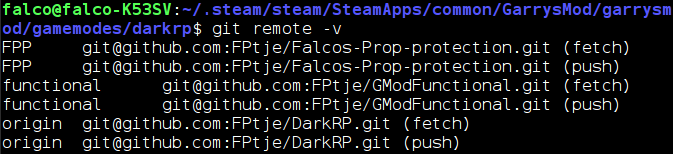
\includegraphics[width=\linewidth]{gitremote.png}
\end{frame}

\subsection{Pushing and pulling}
\begin{frame}[fragile]{Pushing and pulling}
\begin{itemize}
\item push: Push your commits to a branch on a remote
\item pull: Pull commits from a branch on a remote to your local repository
\item git pull = git fetch \&\& git merge
\item \begin{verbatim}git push origin master\end{verbatim}
\item \begin{verbatim}git pull origin master\end{verbatim}
\item Can be shortened to git push and git pull if branch is set to track a remote branch
\begin{verbatim}git branch --set-upstream-to=origin/master\end{verbatim}
\end{itemize}
\end{frame}


\section{Best Practices and tips}
\begin{frame}[fragile]{Best Practices and tips}
\pause
\begin{itemize}
\item \begin{verbatim}alias pw="ssh-add ~/.ssh/id_rsa"\end{verbatim} 
in .bashrc (\href{http://stackoverflow.com/questions/3669001/getting-ssh-agent-to-work-with-git-run-from-windows-command-shell/15870387#15870387}{\color{blue}Windows is slightly annoying here})
\pause
\item ONE commit = ONE thing!!
\pause
\item A commit should NOT break a build completely!
\pause
\item Get familliar with git commands.
\pause
\item Do NOT put ANY compiler generated files in the repository.
\pause
\item Use branches freely (experimental features, a stable branch, big refactors, etc.)
\pause
\item Use git even if you work alone.
\pause
\item Push/pull often enough to prevent conflicts.
\pause
\item Do not change the history of commits that are already pushed to a repository.
\end{itemize}
\end{frame}

\begin{frame}[fragile]{Best Practices and tips}
\begin{itemize}
\item Before committing, always check git status and git diff.
\pause
\item Use private repositories for university projects.
\href{http://git-scm.com/downloads/guis}{\color{blue}https://git.wiki.kernel.org/index.php/GitHosting}
\item Github is awesome for open source projects.
\pause
\item Frightened by terminal commands?
\href{http://git-scm.com/downloads/guis}{\color{blue}http://git-scm.com/downloads/guis} \\
Really, though, the terminal is better than \textit{any} graphical tool.
\pause
\item Oh and whatever you do, don't use tortoisegit. It's even worse than tortoiseSVN.
\end{itemize}
\end{frame}


\section{Awesome things you can do with git}

\subsection{Git revert}
\begin{frame}[fragile]{Git revert}
Creates a commit that undoes another commit.
\begin{verbatim}git revert eff13cb\end{verbatim}
\href{https://www.atlassian.com/git/tutorial/undoing-changes#!revert}{\color{blue}https://www.atlassian.com/git/tutorial/undoing-changes\#!revert}
\href{https://www.kernel.org/pub/software/scm/git/docs/git-revert.html}{\color{blue}https://www.kernel.org/pub/software/scm/git/docs/git-revert.html}

\end{frame}

\subsection{Submodule/Subtree merge}
\begin{frame}{Submodule/Subtree merge}
Have a repository as a subfolder in your repository!

Submodule:
\href{http://git-scm.com/docs/git-submodule}{\color{blue}http://git-scm.com/docs/git-submodule}

Subtree merge:
\href{http://git-scm.com/book/ch6-7.html}{\color{blue}http://git-scm.com/book/ch6-7.html}
\href{https://help.github.com/articles/working-with-subtree-merge}{\color{blue}https://help.github.com/articles/working-with-subtree-merge}
\end{frame}

\subsection{Git bisect}
\begin{frame}{Git bisect}
Binary search for bugs \\
\href{http://git-scm.com/book/en/Git-Tools-Debugging-with-Git\#Binary-Search}{\color{blue}http://git-scm.com/book/en/Git-Tools-Debugging-with-Git\#Binary-Search}
\end{frame}

\subsection{Git tag}
\begin{frame}{Git tag}
Mark release points \\
\href{http://git-scm.com/book/en/Git-Basics-Tagging}{\color{blue}http://git-scm.com/book/en/Git-Basics-Tagging}
\end{frame}

\subsection{Git stash}
\begin{frame}{Git stash}
Store your work for later \\
\href{http://git-scm.com/book/en/Git-Tools-Stashing}{\color{blue}http://git-scm.com/book/en/Git-Tools-Stashing}
\end{frame}

\subsection{Git clean}
\begin{frame}[fragile]{Git clean}
Remove files from the git folder that aren't tracked (or in the .gitignore) \\
Nice alternative for Visual Studio's ``clean solution''. \\
\begin{verbatim}
git clean -xdn
git clean -xdf
\end{verbatim}
\href{https://www.kernel.org/pub/software/scm/git/docs/git-clean.html}{\color{blue}https://www.kernel.org/pub/software/scm/git/docs/git-clean.html}
\end{frame}

\subsection{Git blame}
\begin{frame}[fragile]{Git blame}
\begin{itemize}
\item Much like SVN blame.
\begin{verbatim}git blame file\end{verbatim}
\item Press q to exit the viewer in the terminal.
\end{itemize}
\href{https://www.kernel.org/pub/software/scm/git/docs/git-blame.html}{\color{blue}https://www.kernel.org/pub/software/scm/git/docs/git-blame.html}
\href{http://alblue.bandlem.com/2011/07/git-tip-of-week-assigning-blame.html}{\color{blue}http://alblue.bandlem.com/2011/07/git-tip-of-week-assigning-blame.html}

\end{frame}

\subsection{Pull requests}
\begin{frame}[fragile]{Pull requests}
\begin{itemize}
\item Well implemented by github and gerrit
\item Git has a command for it too
\begin{verbatim}git request-pull origin/master origin\end{verbatim}
\item Tip: When forking a project, work in a topic branch
\item \href{https://help.github.com/articles/using-pull-requests}{\color{blue}https://help.github.com/articles/using-pull-requests}
\item \href{http://git-scm.com/book/ch5-2.html}{\color{blue}http://git-scm.com/book/ch5-2.html}
\end{itemize}
\end{frame}

\begin{frame}{Git request-pull}
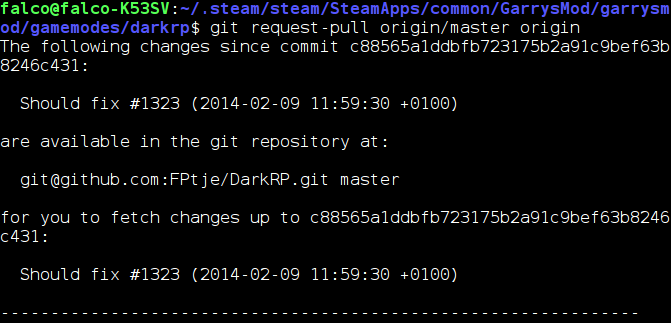
\includegraphics[width=\linewidth]{gitrequestpull.png}
\end{frame}

\begin{frame}{Gerrit (Cyanogenmod)}
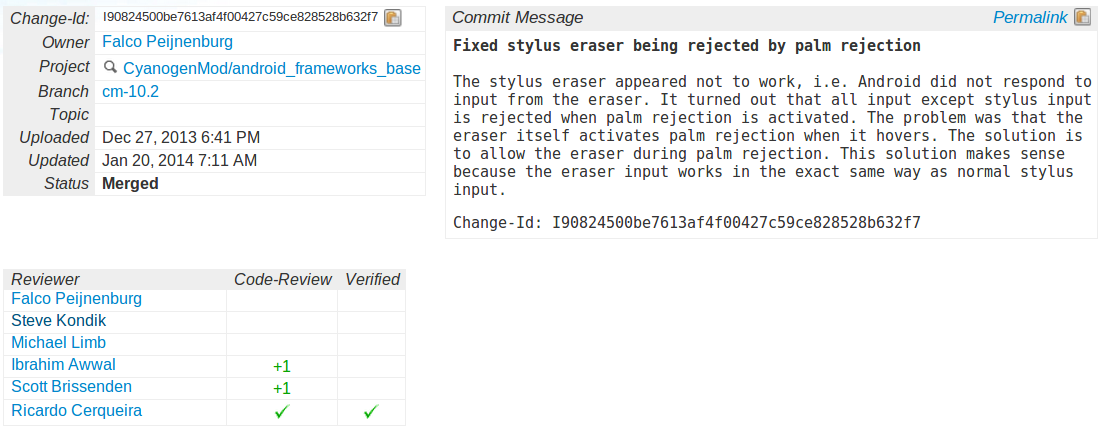
\includegraphics[width=\linewidth]{gerrit.png}
\end{frame}

\begin{frame}{Github pull request}

\includegraphics[width=\linewidth]{githubpull.png}
\end{frame}

\subsection{Cherry-pick}
\begin{frame}{Cherry-pick}
\begin{itemize}
\item Take a single commit from another branch
\item Useful in handling pull requests
\item \href{http://think-like-a-git.net/sections/rebase-from-the-ground-up/cherry-picking-explained.html}{\color{blue}http://think-like-a-git.net/sections/rebase-from-the-ground-up/cherry-picking-explained.html}
\end{itemize}
\end{frame}

\subsection{Set up your own git server}
\begin{frame}{Set up your own git server}
\begin{itemize}
\item \href{http://git-scm.com/book/en/Git-on-the-Server}{\color{blue}http://git-scm.com/book/en/Git-on-the-Server}
\item All you need is a git repository and ssh access to it
\item Knock yourselves out
\end{itemize}
\end{frame}

\section{Further reading}
\begin{frame}
\begin{itemize}
\item Excellent free book: \href{http://git-scm.com/documentation}{\color{blue}http://git-scm.com/documentation}
\item Cheat sheet: \href{http://www.git-tower.com/blog/git-cheat-sheet-detail/}{\color{blue}http://www.git-tower.com/blog/git-cheat-sheet-detail/}
\item Cheat sheet: \href{http://byte.kde.org/~zrusin/git/git-cheat-sheet-medium.png}{\color{blue}http://byte.kde.org/~zrusin/git/git-cheat-sheet-medium.png}
\item Interactive cheat sheet: \href{http://ndpsoftware.com/git-cheatsheet.html}{\color{blue}http://ndpsoftware.com/git-cheatsheet.html}
\item Interactive practical: \href{http://try.github.io/}{\color{blue}http://try.github.io/}
\end{itemize}
\end{frame}

\begin{frame}{Previously posted links}
\begin{itemize}
\item \href{http://git-scm.com/downloads/guis}{\color{blue}https://help.github.com/articles/generating-ssh-keys}
%\item \href{http://git-scm.com/downloads/guis}{\color{blue}https://github.com/github/gitignore}
\item \href{http://stackoverflow.com/questions/3669001/getting-ssh-agent-to-work-with-git-run-from-windows-command-shell/15870387\#15870387}{\color{blue}http://stackoverflow.com/questions/3669001/getting-ssh-agent-to-work-with-git-run-from-windows-command-shell/15870387\#15870387})
\item \href{http://git-scm.com/downloads/guis}{\color{blue}https://git.wiki.kernel.org/index.php/GitHosting}
\item \href{http://git-scm.com/downloads/guis}{\color{blue}http://git-scm.com/downloads/guis} \\
\item \href{https://www.atlassian.com/git/tutorial/undoing-changes\#!revert}{\color{blue}https://www.atlassian.com/git/tutorial/undoing-changes\#!revert}
\item \href{https://www.kernel.org/pub/software/scm/git/docs/git-revert.html}{\color{blue}https://www.kernel.org/pub/software/scm/git/docs/git-revert.html}
\item \href{http://git-scm.com/docs/git-submodule}{\color{blue}http://git-scm.com/docs/git-submodule}
\item \href{http://git-scm.com/book/ch6-7.html}{\color{blue}http://git-scm.com/book/ch6-7.html}
\item \href{https://help.github.com/articles/working-with-subtree-merge}{\color{blue}https://help.github.com/articles/working-with-subtree-merge}
\item \href{http://git-scm.com/book/en/Git-Tools-Debugging-with-Git\#Binary-Search}{\color{blue}http://git-scm.com/book/en/Git-Tools-Debugging-with-Git\#Binary-Search}
\end{itemize}
\end{frame}

\begin{frame}{Previously posted links}
\begin{itemize}
\item \href{http://git-scm.com/book/en/Git-Basics-Tagging}{\color{blue}http://git-scm.com/book/en/Git-Basics-Tagging}
\item \href{http://git-scm.com/book/en/Git-Tools-Stashing}{\color{blue}http://git-scm.com/book/en/Git-Tools-Stashing}
\item \href{https://www.kernel.org/pub/software/scm/git/docs/git-clean.html}{\color{blue}https://www.kernel.org/pub/software/scm/git/docs/git-clean.html}
\item \href{https://www.kernel.org/pub/software/scm/git/docs/git-blame.html}{\color{blue}https://www.kernel.org/pub/software/scm/git/docs/git-blame.html}
\item \href{http://alblue.bandlem.com/2011/07/git-tip-of-week-assigning-blame.html}{\color{blue}http://alblue.bandlem.com/2011/07/git-tip-of-week-assigning-blame.html}
\item \href{https://help.github.com/articles/using-pull-requests}{\color{blue}https://help.github.com/articles/using-pull-requests}
\item \href{http://git-scm.com/book/ch5-2.html}{\color{blue}http://git-scm.com/book/ch5-2.html}
\item \href{http://think-like-a-git.net/sections/rebase-from-the-ground-up/cherry-picking-explained.html}{\color{blue}http://think-like-a-git.net/sections/rebase-from-the-ground-up/cherry-picking-explained.html}
\item \href{http://git-scm.com/book/en/Git-on-the-Server}{\color{blue}http://git-scm.com/book/en/Git-on-the-Server}
\end{itemize}
\end{frame}

\end{document}